% THIS IS AN EXAMPLE DOCUMENT FOR VLDB 2012
% based on ACM SIGPROC-SP.TEX VERSION 2.7
% Modified by  Gerald Weber <gerald@cs.auckland.ac.nz>
% Removed the requirement to include *bbl file in here. (AhmetSacan, Sep2012)
% Fixed the equation on page 3 to prevent line overflow. (AhmetSacan, Sep2012)

\documentclass{vldb}
\usepackage{algorithm}
\usepackage{algorithmic}
\usepackage{graphicx}
\usepackage{multirow} %multirow for format of table 
\usepackage{amsmath} 
\usepackage{xcolor}
\usepackage{balance}  % for  \balance command ON LAST PAGE  (only there!)


\begin{document}

% ****************** TITLE ****************************************
\title{Cost-based Pivot Selection for Similarity Search in Large Relation Databases }

\numberofauthors{8} 
\author{
\alignauthor
Ben Trovato\titlenote{Dr.~Trovato insisted his name be first.}\\
       \affaddr{Institute for Clarity in Documentation}\\
       \affaddr{1932 Wallamaloo Lane}\\
       \affaddr{Wallamaloo, New Zealand}\\
       \email{trovato@corporation.com}
% 2nd. author
\alignauthor
G.K.M. Tobin\titlenote{The secretary disavows
any knowledge of this author's actions.}\\
       \affaddr{Institute for Clarity in Documentation}\\
       \affaddr{P.O. Box 1212}\\
       \affaddr{Dublin, Ohio 43017-6221}\\
       \email{webmaster@marysville-ohio.com}
% 3rd. author
\alignauthor Lars Th{\Large{\sf{\o}}}rv{$\ddot{\mbox{a}}$}ld\titlenote{This author is the
one who did all the really hard work.}\\
       \affaddr{The Th{\large{\sf{\o}}}rv{$\ddot{\mbox{a}}$}ld Group}\\
       \affaddr{1 Th{\large{\sf{\o}}}rv{$\ddot{\mbox{a}}$}ld Circle}\\
       \affaddr{Hekla, Iceland}\\
       \email{larst@affiliation.org}
\and  % use '\and' if you need 'another row' of author names
% 4th. author
\alignauthor Lawrence P. Leipuner\\
       \affaddr{Brookhaven Laboratories}\\
       \affaddr{Brookhaven National Lab}\\
       \affaddr{P.O. Box 5000}\\
       \email{lleipuner@researchlabs.org}
% 5th. author
\alignauthor Sean Fogarty\\
       \affaddr{NASA Ames Research Center}\\
       \affaddr{Moffett Field}\\
       \affaddr{California 94035}\\
       \email{fogartys@amesres.org}
% 6th. author
\alignauthor Charles Palmer\\
       \affaddr{Palmer Research Laboratories}\\
       \affaddr{8600 Datapoint Drive}\\
       \affaddr{San Antonio, Texas 78229}\\
       \email{cpalmer@prl.com}
}

\additionalauthors{Additional authors: John Smith (The Th{\o}rv\"{a}ld Group, {\texttt{jsmith@affiliation.org}}), Julius P.~Kumquat
(The \raggedright{Kumquat} Consortium, {\small \texttt{jpkumquat@consortium.net}}), and Ahmet Sacan (Drexel University, {\small \texttt{ahmetdevel@gmail.com}})}
\date{30 July 1999}




\maketitle
\newtheorem{myDef}{Definition} 
\newtheorem{myTheo}{Theorem}
\newtheorem{lem}{Lemma}
%\documentclass[journal]{IEEEtran}

%\usepackage{algpseudocode}
%\usepackage{amsmath}
%\usepackage{graphics}
%\usepackage{epsfig}
\begin{abstract}
The abstract for your paper for the PVLDB Journal submission.
The template and the example document are based on the ACM SIG Proceedings  templates. This file is part of a package for preparing the submissions for review. These files are in the camera-ready format, but they do not contain the full copyright note.
Note that after the notification of acceptance, there will be an updated style file for the camera-ready submission containing the copyright note.
\end{abstract}




\section{Introduction}
Similarity search is a primitive operation that is at the heart of a wide spectrum of database applications, including face recognition, fingerprint matching in multimedia databases, location based services in spatial databases, error checking in text retrieval, pattern recognition (e.g. DNA or Protein sequences) in computational biology, etc.

Lots of indexing methods based on the properties of metric spaces have been developed to efficiently solve similarity search. These methods are usually classified in pivot   based (which store precomputed distances to discard objects) or clustering   based algorithms (which partition the space into clusters to discard some of them during the search). The work presented in this paper is focused on the case of pivot-based algorithms.

The rationale behind pivot based method is to first select m objects as pivots and then assign each object to a single pivot according to a certain strategy. After the assignment is completed, the whole data space is split into m disjoint partitions. Within each partition, the distances from objects to pivot are also maintained. Then, similarity queries can be efficiently processed by examining each partition individually. Following the filtering-and- verification paradigm, the similar objects within each partition can be determined according to the triangle inequality. Finally, each of the candidates is verified and similar objects are returned.

Pivot-based methods are widely used to process similarity queries in metric spaces, e.g. Mtree, iDistance and PBI. In iDistance, object r is assigned to its closest pivot or furthest pivot, while in PBI, object r is assigned to the pivot that maximizes the probability of r being pruned with respect to a given query workload. The majority of existing solutions focus on either designing new index structures associated with new index probing algorithms or developing new index probing algorithms with existing indices, as native engines to improve efficiency. However, all of existing solutions do not address how to determine the optimal pivot number. They just take pivot number as the tuning parameter and experimental results are obtained with the optimal pivot number, which makes contrast experiments incomparable. Therefore, how to determine the optimal pivot number still remains open and it is a worth studying problem to be solved.

The performance of pivot-based method depends on the pivot selection. The way to choose pivots and how to determine the number of pivots are of significance to the time of query process. The way to choose pivots influences the positions of pivots in the space so that it determines the capacity  of the index to discard objects without comparing them with the query. Other important issue is how to determine the optimal pivot number. As shown in figure 1, with the increase of pivot number, query time first decreases and then increases. The reason is that the query has to be compared with both the pivots in main memory (internal complexity) and the objects in disk that can not be discarded (external complexity), so we have to reach a good trade-off between the number of pivots and their power of filtering.

\begin{figure}[ht]
\centering
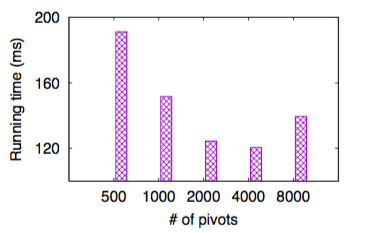
\includegraphics[width=8cm,height=7cm]{pivot}
\caption{Query Time With Different Pivot Number}
\label{fig:stream}
\end{figure}

So far, a variety of pivot-based methods have been proposed to perform similarity research such as SSS, FFT and so on. However, there still remains some shortness with respect to these issues:
\begin{itemize}
\item What most of the pivot based algorithms have in common is that they determine the optimal pivot number through a large number of experiments, thus causing high cost and making contrast experiment incomparable.
\end{itemize}
\begin{itemize}
\item From our observation, we conclude that the number of pivots usually plays a role that is not less important than the  way to choose pivots to determine the performance of pivot-based method. Sometimes, the distinction in query time between different methods is less than that between different pivot number. Most existing pivot-based methods just take the pivot number as tuning parameter, which may cause the slip of opportunity to enhance the performance of query processes largely in the real application. 
\end{itemize}
In this paper, we propose a cost-based pivot selection strategy which can dynamically select the optimal number of pivots.According to our research , impact factors of query time are dataset size, pivot number and similarity function. Given a collection of objects R and a query workload, we can get its cost model using the cost-based pivot selection strategy, whose parameters are determined by above factors. In this way, for any size of dataset R, we can immediately get its optimal point number through the cost model. Besides, when dataset R increases or decreases, the optimal point number will change correspondingly. Therefore, we propose an update mechanism, that is, when the size of R changes, point number and the index will be adjusted dynamically according to cost model, which makes the query in an optimal state.
In summary, our contributions are as follows:
\begin{itemize}
\item To the best of our knowledge, this paper first proposes a way to access the expected query time for a certain pivot number. It provides a generic method which is suitable for any type of data. Then, algorithm for finding optimal pivot number are given.
\end{itemize}

\begin{itemize}
\item Our work can be integrated into existing RDBMS,
which makes our work has good generality.
\end{itemize}
\begin{itemize}
\item We deploy methods proposed in this paper on top of PostgreSQL and conduct extensive experiments on various real data sets. These experiments demonstrate the benefits of our work.
\end{itemize}
The rest of the paper is organized as follows. Section 2 states the problem and necessary definitions. Section 3 gives an overview of cost-based pivot selection for optimal pivot number. Experimental results are presented in Section 4. Finally,Section 5 concludes the paper.

\begin{table*}
\centering
\caption{Some Typical Commands}
\begin{tabular}{|l||l|} 
\hline
D & a metric space  \\
\hline
R & the input dataset R  \\
\hline
S&  a sample of R   \\
\hline
U&  a universal string domain   \\
\hline

 $\theta$& a query threshold  \\
\hline
$|r,r'|$& the distance between two objects r and r' \\
\hline
q& a query object in D \\
\hline
$\mathbb{P}$ & a set of pivots\\
\hline
$P_i$& a pivot in $\mathbb{P}$ \\
\hline
pnum & the number of pivots \\
\hline
$con_i$&  candidates in $P_i$  \\
\hline
MC(r,r')&  time for measuring the distance between disk resident strings   \\
\hline
DC(r,r')&  time for measuring the distance between main memory strings \\
\hline
sim&  similarity function,such as Edit-distance for text space and L1 for dimension space \\
\hline
simCost(d,sim)& time for using sim to measure distance between main memory strings with d as the average length of strings    \\
\hline
m& time of measuring distance between disk resident strings is as m times large as that of main memory strings \\
\hline
$T_c$& time of range generation\\
\hline
$T_v$& time of candidate verification\\
\hline
\end{tabular}
\end{table*}





\section{ PROBLEM  DEFINTION}

\begin{myDef}[Similarity Search ]
Given a query object q, a data set R, and a threshold , the similarity search identifies objects $\{r|r\in R ,|r-q|<\theta \}$ in R with distance to q less than or equal to a user-defined threshold $\theta$.
\end{myDef}

\begin{myTheo}
Given a partition $P_i$, ${\forall r \in P_i}$, the necessary condition that $|q,r| \le \theta$ is:
$$|p_i,q|- \theta \le |p_i,r| \le |p_i,q|+ \theta$$
\end{myTheo}
When the whole data set is split into disjoint partitions, similarity queries can be efficiently processed by examining each partition $P_i$ individually. Then, following the filtering-and-verification paradigm, the similar objects within $P_i$ can be determined. The filtering rule is based on Theorem 1, in which ${\forall r \in P_i}$, $|r,p_i| \in [|p_i,q| -\theta,p_i,q|+ \theta]$ are taken as candidates. Finally, each of the candidates is verified and similar objects are returned.

\begin{myDef}[query time]
Given a dataset R, and a query q, the query time consists of two parts:
Search range generation and Candidate verification.
\begin{itemize}
\item  Range generation: time that q compared with pivots, determined by pivot number and similarity function. 
\item  Candidate verification: time that q compared with the objects that can not be discarded, determined by database size, pivot number and similarity function.
\end{itemize}
\end{myDef}
Let Qtime(q) be the query time of q, $MC(p_i,q)$ be the time for measuring distance between $p_i$ and q,  $DC(r_j,q)$ be the time for measuring distance between $r_j$ and q. Because both query and pivots are main memory data and candidates are disk resident data. It is noted that $MC(p_i,q)$ is usually smaller than $DC(r_j,q)$.

\begin{equation}Qtime(q)=\sum_{i=1}^{Pnum}MC(\mathnormal{p}_i,q)+ \sum_{i=1}^{Pnum}\sum_{r_j \in con_i}DC(r_j,q) \end{equation}
Furthermore,let d be the average length of strings in database R and $|can_i|$ be the number of candidates in $P_i^R$ . Without loss of generality, we can use simCost(d,sim) to denote the time for measuring distance between two strings of the database R with d as average length in main memory and $m*simCost(d,sim)$ to denote the time for measuring distance between two strings of the database R from disk. And m is a constant number that is usually bigger than one. We can get m through experiment. 
So  Qtime(q) can be illustrated:
\begin{equation}Qtime(q)=(pnum+ m* \sum_{i=1}^{Pnum}|con_i|)*simCost(d,sim)\end{equation}


\begin{myDef}[average filtering ability]
Filtering ability indicates the 
possibility of a string being filtered in the filtering stage in a certain partition. Average filtering ability demonstrates the average possibility of a string being filtered in database R, when a query workload is given. 
\end{myDef}
Average filtering ability has a strong bond with the the pivot set $\mathbb{P}$.As we can select $\mathbb{P}$ for a certain pivot number using the pivot-based method like PBI or Maximum Variance, we can say that the average filtering ability for a certain pivot-based method in database R is a function of pivot number.
\begin{equation}average \;filtering \;ability= FI(pnum)\end{equation}
So the average query time can be expressed as blow:
\begin{equation}Qtime=\lbrack \ pnum+m*(1-FI(pnum))*|R| \ \rbrack*simCost(d,sim)\end{equation}

\begin{myDef}[optimal pivot number]
 The higher the number of pivots is,the more time range generation takes while the less time candidate verification takes. Therefore, it is important to reach a good trade-off between the number of pivots and their power of discrimination. The optimal point number is the number of pivots that  minimizes the query time.
\end{myDef}
\textbf{Problem Statement}
Unless otherwise specified, any object or data set we mention in the paper lies in the metric space \textit{D}. Without loss of generality, given a database R,our mission is to seek a way to find the optimal pivot number for existing pivot-based method at acceptable cost.
According to equation $(4)$, if we want to get the optimal pivot number, only $ \ pnum+m*(1-FI(pnum))*|R| \ $, say Q(pnum), will play a difference, because $simCOSt(d,sim)$ is a constant for a certain database and similarity function.
\begin{equation}Q(pnum)=\ pnum+m*(1-FI(pnum))*|R| \end{equation}
So our task can convert into how to obtain the Q(pnum) for different pivot number. As m is a constant that can be get through experiments, so the only thing we need to know is the relationship between average filtering ability and pivot number.
\section{Optimal Pivot Number Determination}


Given a pivot p, let $f_p(q,i)$ be the probability density function (PDF) over a universal string domain U that describe the probability that $|p,q|=i, \forall q \in U$.
Formally,
\begin{equation}f_p(q,i)=\frac{|\{q|\forall q \in R, |p,q|=i\}|}{|R|}\end{equation}
Deriving the actual PDF of each pivot p for a universal string domain U is impossible. Hence, we approximate the PDF by using a sample of U instead of U. In practice, we can also approximate $f_p(q,i)$ after collecting a proper number of queries and using these queries as U. 

\begin{lem}[Relative Verification Likelihood]
Given a string r that belongs to partition P, when we issue a range query with threshold $\theta$, the likelihood that r needs to be verified with respect to its corresponding pivot p is:
\begin{equation}\rho(r)=\sum_{L\le i \le U} f_p(q,i)\end{equation}
where $L=|p,q|-\theta$, $U=|p,q|+\theta$
\end{lem}
The above equation expresses the likelihood that r will have to be verified with respect to pivot p.Therefore, given a database R and pivot number, the expected number of strings in R that need to be verified is: 
\begin{equation}E(R)=\sum_{r \in R}\rho(r)\end{equation}

\begin{lem}[average filtering ability]
As calculate E(R) is very costly, so we can use a sample of R, say S. So give pivot number, the average filtering ability over database is:
\begin{equation}FI(pnum)=1-\frac{E(S)}{|S|}\end{equation}
\end{lem}
When we increase the number of pivots, the average filtering ability will increase in general, but the speed of increasing will decrease.  In the meanwhile,  pnum will increase but the speed of its increase will certainly remain constant. So according to $(5)$ we can conclude that Q(pnum) will fist decrease than increase, with the increasing of pivot number . If we want to figure out the optimal pivot number, the simple and  natural thought is that we increase pivot number until Q(pnum) decreases. The algorithm is demonstrated as follows: 

\begin{algorithm}
	\caption{OriginalOPnum$(R)$}
	\begin{algorithmic}[1]
		\STATE $i=0$	
        \STATE Calculate $Q(0)$                \REPEAT
        \STATE i=i+1
        \STATE Calculate Q(i)
      \UNTIL{$Q(i)<Q(i-1)$}
        \RETURN i-1
	\end{algorithmic}
\end{algorithm}
But in reality, Q(pnum) may not only have one minimal value, because of the uncertainty in average filtering ability. If that happens, we may stop early before we find the optimal pivot number, when using OriginalOpnum(R).  So we can adopt Simulated Annealing method to find the minimum value:
\begin{algorithm}
	\caption{SimulatedAnnealOpnum$(R,step)$}
	\begin{algorithmic}[1]
		\STATE x=step	
        \WHILE{step<=01 }
           \IF{Q(x-step)<Q(x)}
              \STATE x=x-step
               \ENDIF
            \IF{Q(x+step)<Q(x)}
               \STATE x=x+step
            \ENDIF
            \STATE $step=step-1$
        \ENDWHILE
        \RETURN x
	\end{algorithmic}
\end{algorithm}

In SimulatedAnnealOpnum$(R,step)$, we set the value of step according to the size of database R. 
\end{document}
